\documentclass[12pt]{article}
\usepackage[spanish]{babel}
\usepackage[utf8]{inputenc}
\usepackage{amsmath, amssymb, amsfonts}
\usepackage{graphicx}
\graphicspath{{./EDOs_imgs}}
\usepackage[margin=2.54cm]{geometry}
\usepackage{setspace}
\usepackage{fancyhdr}
\usepackage{titlesec}
\usepackage{apacite}
\usepackage{hyperref}
\usepackage{float}
\usepackage{tikz}
\usepackage{mathtools}

\pagestyle{fancy}
\fancyhf{}
\rhead{\thepage}
\renewcommand{\headrulewidth}{0pt}

%
% \doublespacing
% \setlength{\parindent}{0.5in}

% \titleformat{\section}{\normalfont\large\bfseries}{\thesection}{1em}{}
% \titleformat{\subsection}{\normalfont\normalsize\bfseries}{\thesubsection}{1em}{}

% \title{
%     \vspace{2cm}
%     \Large\textbf{Ecuaciones Diferenciales Homogéneas y Coeficientes Lineales: Aplicaciones en Ingeniería de Sistemas}
%     \vspace{1cm}
% }

% \author{
%     Autor 1 \\
%     Autor 2 \\
%     Ingeniería de Sistemas, Universidad ejemplo \\
% }
% \date{\today}

\begin{document}


\begin{titlepage}
    \centering
    \vspace*{2cm}
    
    {\LARGE \textbf{Ecuaciones Diferenciales Homogéneas y Coeficientes Lineales: Aplicaciones en Ingeniería de Sistemas}\par}
    
    \vspace{3cm}
    
    {\large Julio Cesar Amaya Amaya \\ Danny José Hernández González\par}
    \vspace{0.5cm}
    {\large Ingeniería de Sistemas, Universidad de la Guajira\par}
    
    \vspace{2cm}
    
    {\large \today\par}
    
    \vspace{3cm}
    
    \begin{flushleft}
        Trabajo presentado para el curso de Ecuaciones Diferenciales\\
        Grupo: C2\\
        Profesor: Yoni Cotez Gualé
    \end{flushleft}
    
    \vfill
\end{titlepage}

% \maketitle
\thispagestyle{empty}
% \vfill
% \begin{center}
%     \textbf{Resumen}
% \end{center}
% \begin{quote}
%     Las ecuaciones diferenciales homogéneas con coeficientes lineales constituyen una herramienta fundamental en el modelado matemático de sistemas dinámicos. Este documento presenta una revisión teórica y aplicada de estos conceptos, enfatizando su relevancia en el ámbito de la Ingeniería de Sistemas. Se abordan métodos de solución analíticos y se ilustran aplicaciones prácticas en control automático, redes de comunicación y simulación de procesos. Los ejemplos resueltos demuestran la utilidad de estas ecuaciones para describir comportamientos temporales en sistemas complejos.
% \end{quote}
\newpage

\section{Introducción}

Las ecuaciones diferenciales homogéneas con coeficientes lineales representan una clase fundamental de ecuaciones que modelan fenómenos dinámicos en múltiples disciplinas de la ingeniería. En el contexto de la Ingeniería de Sistemas, estas ecuaciones son particularmente relevantes para describir y analizar el comportamiento temporal de sistemas complejos, desde redes de computadoras hasta procesos de manufactura automatizada.

La importancia de estas ecuaciones radica en su capacidad para capturar relaciones causa-efecto en sistemas donde las tasas de cambio dependen linealmente del estado actual. Por ejemplo, en sistemas de control automático, las ecuaciones diferenciales homogéneas permiten modelar la respuesta temporal de controladores PID, la dinámica de sistemas mecánicos amortiguados, o la propagación de señales en redes de comunicación.

En el ámbito de la simulación de procesos, estas ecuaciones permiten predecir el comportamiento de sistemas bajo diferentes condiciones iniciales, facilitando la optimización de parámetros y la identificación de posibles fallos antes de la implementación física. La capacidad de resolver analíticamente estas ecuaciones proporciona una ventaja significativa en términos de comprensión del sistema y predicción de su comportamiento a largo plazo.

Este documento presenta una revisión sistemática de los conceptos teóricos fundamentales relacionados con ecuaciones diferenciales homogéneas con coeficientes lineales, sus métodos de solución, y aplicaciones prácticas específicas en Ingeniería de Sistemas. El enfoque se centra en proporcionar herramientas matemáticas que permitan a los ingenieros modelar, analizar y predecir el comportamiento de sistemas dinámicos complejos.

\section{Desarrollo}

\subsection{Conceptos Fundamentales}

Una ecuación diferencial homogénea con coeficientes lineales es una ecuación de la forma:

\begin{equation}
    a_n \frac{d^n y}{dx^n} + a_{n-1} \frac{d^{n-1} y}{dx^{n-1}} + \cdots + a_1 \frac{dy}{dx} + a_0 y = 0
\end{equation}

donde $a_0, a_1, \ldots, a_n$ son coeficientes constantes y $y$ es una función de $x$.

\subsection{Ecuaciones de Segundo Orden}

Para el caso particular de ecuaciones de segundo orden, la forma general es:

\begin{equation}
    a \frac{d^2 y}{dx^2} + b \frac{dy}{dx} + c y = 0
\end{equation}

La solución se obtiene mediante la ecuación característica:

\begin{equation}
    ar^2 + br + c = 0
\end{equation}

Las raíces de esta ecuación determinan la forma de la solución general:

\textbf{Caso 1: Raíces reales distintas} ($b^2 - 4ac > 0$)
\begin{equation}
    y(x) = C_1 e^{r_1 x} + C_2 e^{r_2 x}
\end{equation}

\textbf{Caso 2: Raíces reales repetidas} ($b^2 - 4ac = 0$)
\begin{equation}
    y(x) = (C_1 + C_2 x) e^{rx}
\end{equation}

\textbf{Caso 3: Raíces complejas conjugadas} ($b^2 - 4ac < 0$)
\begin{equation}
    y(x) = e^{\alpha x} (C_1 \cos(\beta x) + C_2 \sin(\beta x))
\end{equation}

\subsection{Aplicación en Sistemas de Control}

En sistemas de control automático, las ecuaciones diferenciales homogéneas modelan la respuesta natural de sistemas de segundo orden. Consideremos un sistema masa-resorte-amortiguador:

\begin{equation}
    m \frac{d^2 x}{dt^2} + c \frac{dx}{dt} + kx = 0
\end{equation}

donde $m$ es la masa, $c$ es el coeficiente de amortiguamiento, y $k$ es la constante del resorte.

La solución de esta ecuación describe el comportamiento transitorio del sistema, crucial para determinar estabilidad y tiempo de respuesta en sistemas de control.

\subsection{Análisis de Redes de Comunicación}

En el modelado de redes de comunicación, las ecuaciones diferenciales homogéneas describen la dinámica de colas y la propagación de señales. Para un sistema de cola M/M/1, la ecuación de estado puede formularse como:

\begin{equation}
    \frac{dP_n(t)}{dt} = \lambda P_{n-1}(t) - (\lambda + \mu) P_n(t) + \mu P_{n+1}(t)
\end{equation}

En estado estacionario, esta ecuación se simplifica a un sistema homogéneo que permite analizar la estabilidad de la red.

\section{Ejercicios}

\subsection{Ejercicio 1: Sistema Masa-Resorte-Amortiguador}

Resolver la ecuación diferencial que modela un sistema masa-resorte-amortiguador con $m = 2$ kg, $c = 8$ Ns/m, y $k = 32$ N/m, con condiciones iniciales $x(0) = 0.1$ m y $x'(0) = 0$ m/s.

\textbf{Solución:}
La ecuación diferencial es:
\begin{equation}
    2 \frac{d^2 x}{dt^2} + 8 \frac{dx}{dt} + 32x = 0
\end{equation}

Simplificando:
\begin{equation}
    \frac{d^2 x}{dt^2} + 4 \frac{dx}{dt} + 16x = 0
\end{equation}

La ecuación característica es:
\begin{equation}
    r^2 + 4r + 16 = 0
\end{equation}

Las raíces son: $r = -2 \pm 2\sqrt{3}i$

La solución general es:
\begin{equation}
    x(t) = e^{-2t} (C_1 \cos(2\sqrt{3}t) + C_2 \sin(2\sqrt{3}t))
\end{equation}

Aplicando las condiciones iniciales:
\begin{align}
    x(0) &= C_1 = 0.1 \\
    x'(0) &= -2C_1 + 2\sqrt{3}C_2 = 0 \Rightarrow C_2 = \frac{0.2}{2\sqrt{3}} = \frac{0.1}{\sqrt{3}}
\end{align}

La solución particular es:
\begin{equation}
    x(t) = e^{-2t} \left(0.1 \cos(2\sqrt{3}t) + \frac{0.1}{\sqrt{3}} \sin(2\sqrt{3}t)\right)
\end{equation}

\begin{figure}[H]
    \centering
    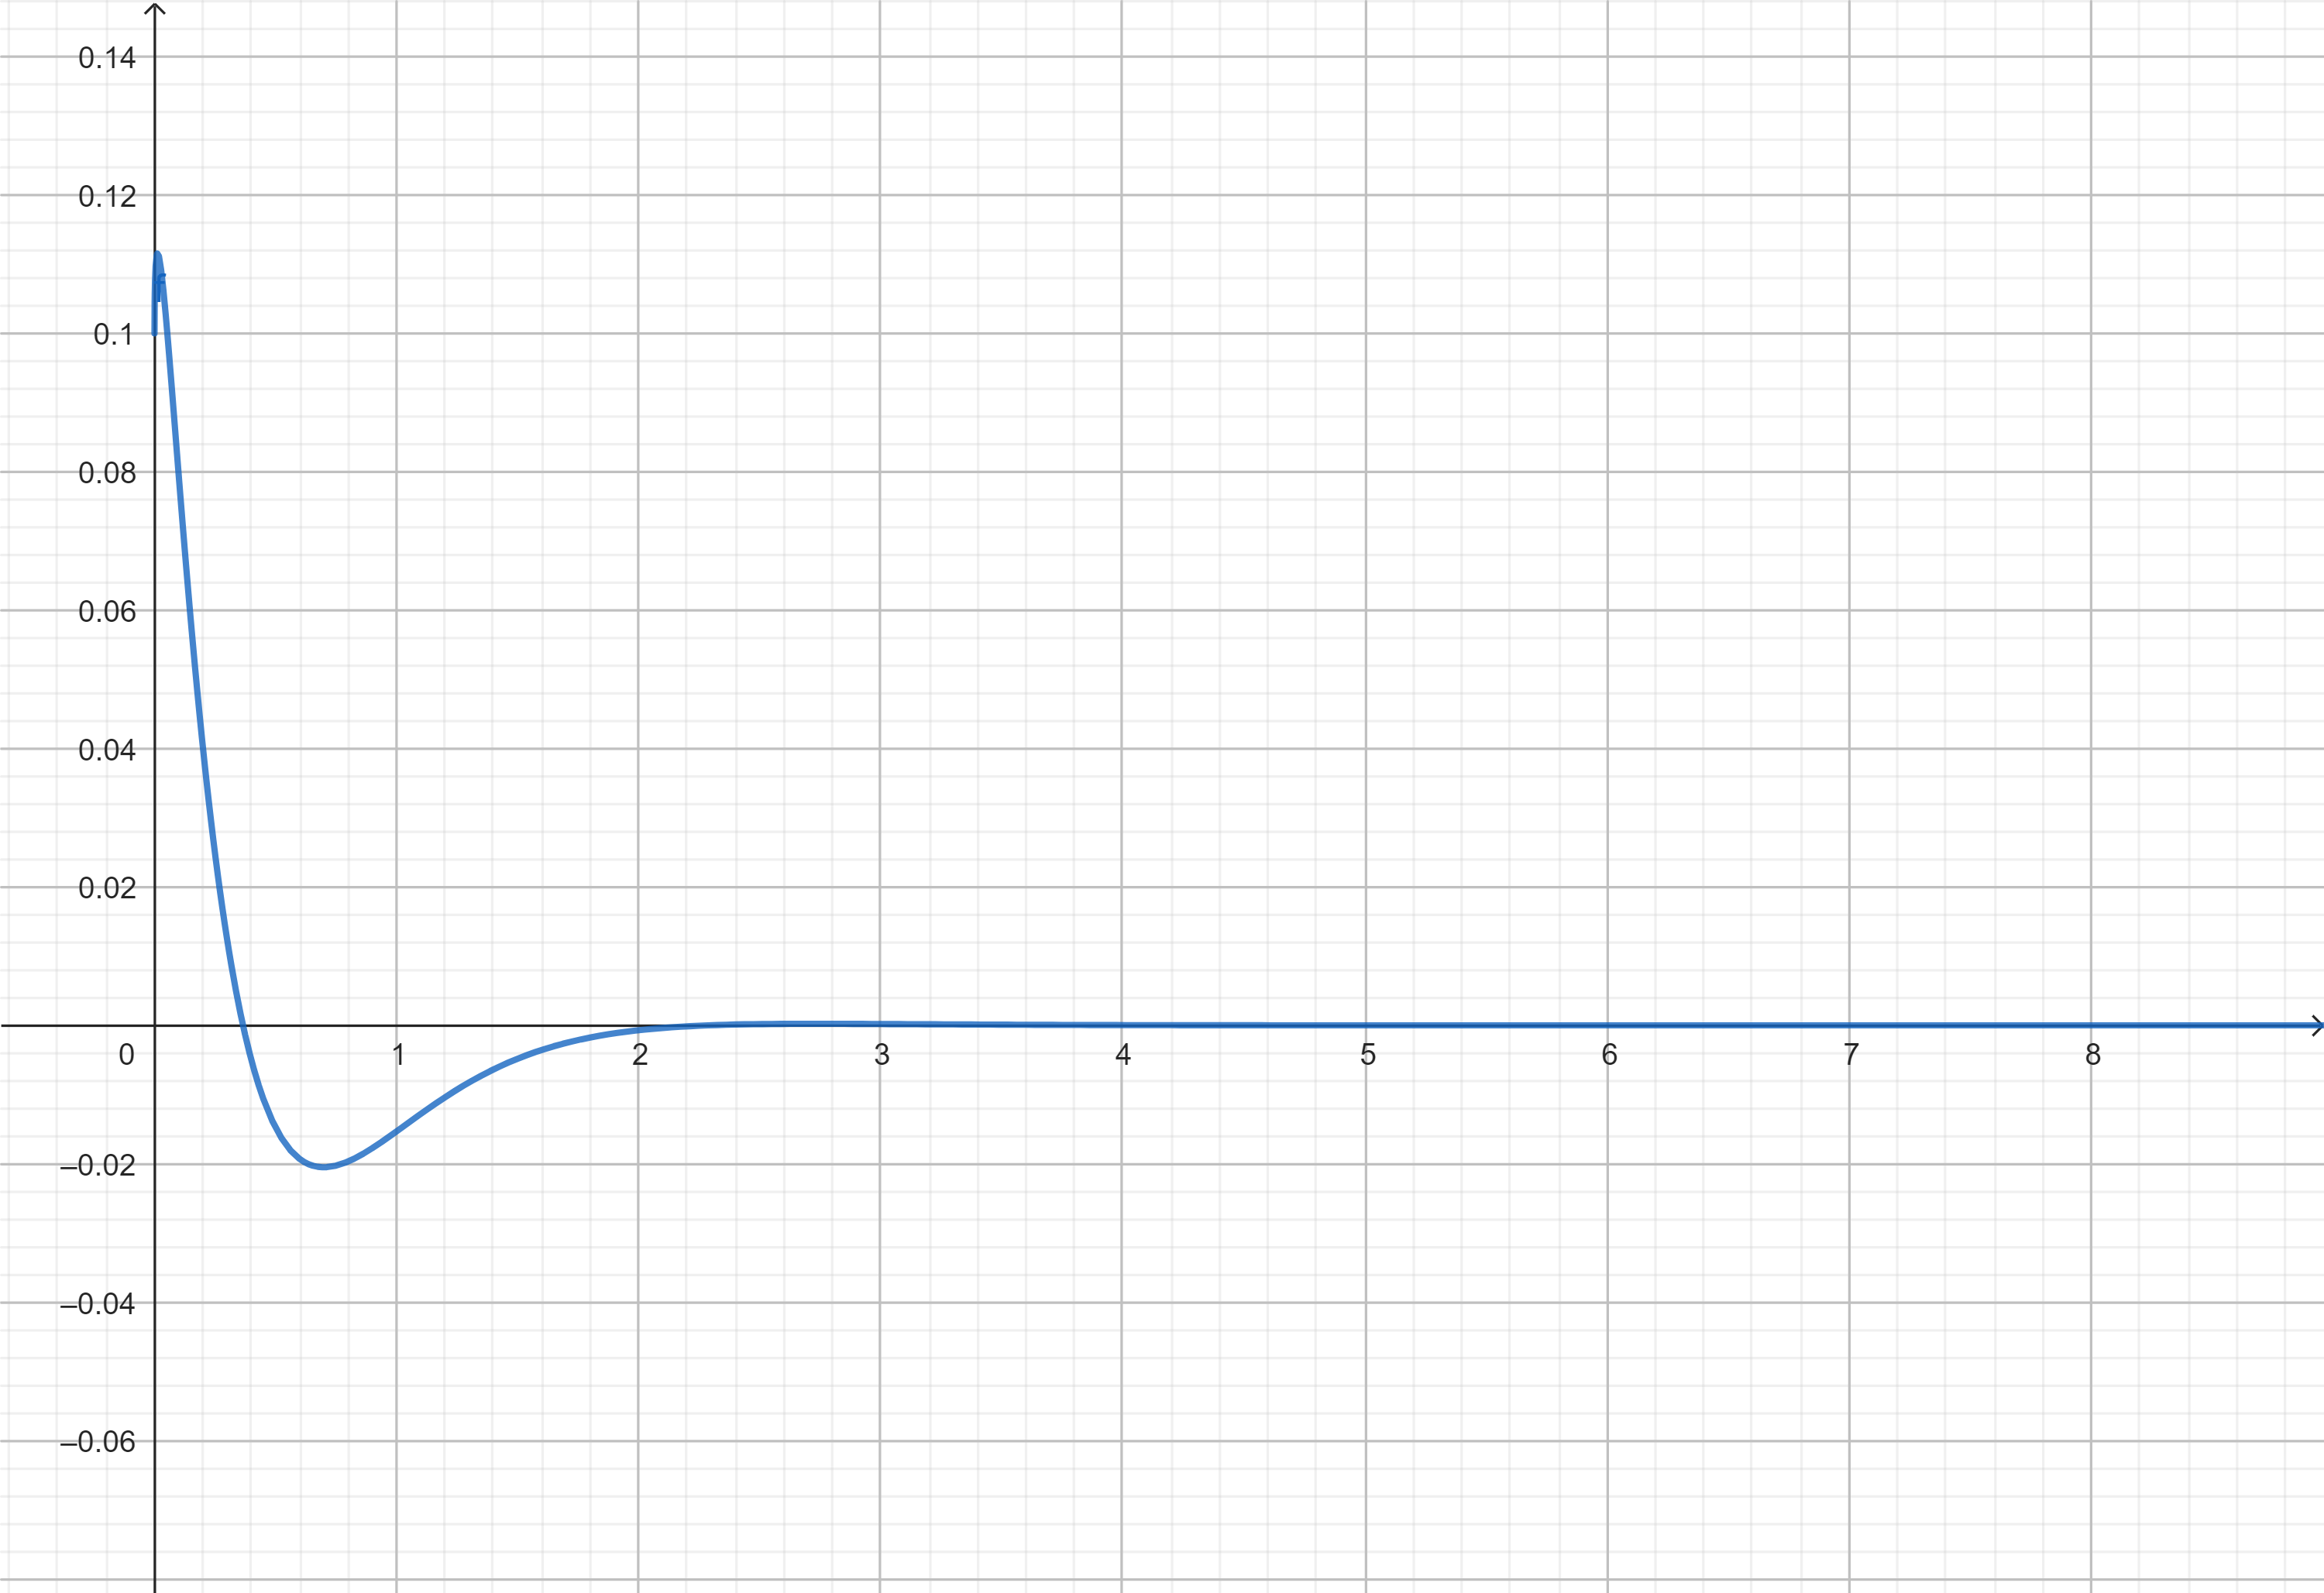
\includegraphics[width=0.8\textwidth]{imagen-ejercicio1.png}
    \caption{Respuesta temporal del sistema masa-resorte-amortiguador obtenida con GeoGebra}
\end{figure}

\subsection{Ejercicio 2: Circuito RLC en Serie}

Un circuito RLC en serie tiene $R = 100$ Ω, $L = 0.5$ H, y $C = 10$ μF. Determinar la corriente $i(t)$ si la fuente de voltaje se retira repentinamente y $i(0) = 0.1$ A, $\frac{di}{dt}(0) = 0$.

\textbf{Solución:}
La ecuación del circuito es:
\begin{equation}
    L \frac{d^2 i}{dt^2} + R \frac{di}{dt} + \frac{1}{C} i = 0
\end{equation}

Sustituyendo valores:
\begin{equation}
    0.5 \frac{d^2 i}{dt^2} + 100 \frac{di}{dt} + 10^5 i = 0
\end{equation}

La ecuación característica es:
\begin{equation}
    0.5r^2 + 100r + 10^5 = 0
\end{equation}

Las raíces son: $r = -100 \pm 400i$

La solución es:
\begin{equation}
    i(t) = e^{-100t} (C_1 \cos(400t) + C_2 \sin(400t))
\end{equation}

Aplicando condiciones iniciales:
\begin{align}
    i(0) &= C_1 = 0.1 \\
    \frac{di}{dt}(0) &= -100C_1 + 400C_2 = 0 \Rightarrow C_2 = 0.025
\end{align}

\begin{figure}[H]
    \centering
    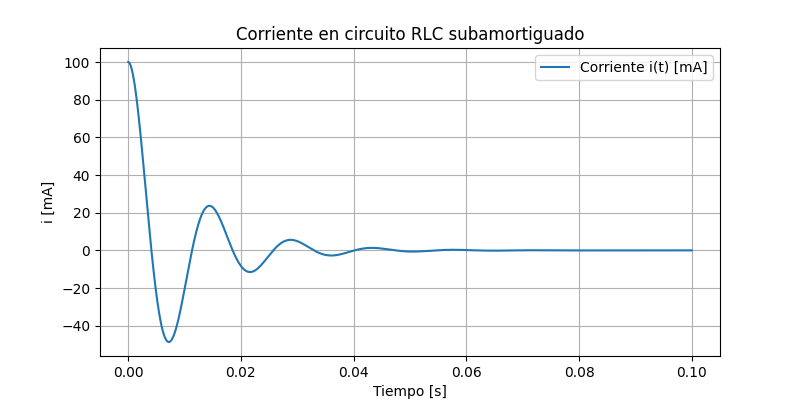
\includegraphics[width=0.8\textwidth]{imagen-ejercicio2.png}
    \caption{Corriente en el circuito RLC obtenida mediante simulación en Python}
\end{figure}

\subsection{Ejercicio 3: Sistema de Control de Nivel}

Un tanque de almacenamiento tiene una dinámica descrita por:
\begin{equation}
    A \frac{dh}{dt} = -k h
\end{equation}

donde $A = 5$ m² es el área transversal y $k = 0.5$ m²/s es el coeficiente de salida. Resolver para $h(t)$ con $h(0) = 2$ m.

\textbf{Solución:}
La ecuación se simplifica a:
\begin{equation}
    \frac{dh}{dt} + \frac{k}{A} h = 0
\end{equation}

Esta es una ecuación de primer orden homogénea con solución:
\begin{equation}
    h(t) = h(0) e^{-\frac{k}{A}t} = 2 e^{-0.1t}
\end{equation}

\begin{figure}[H]
    \centering
    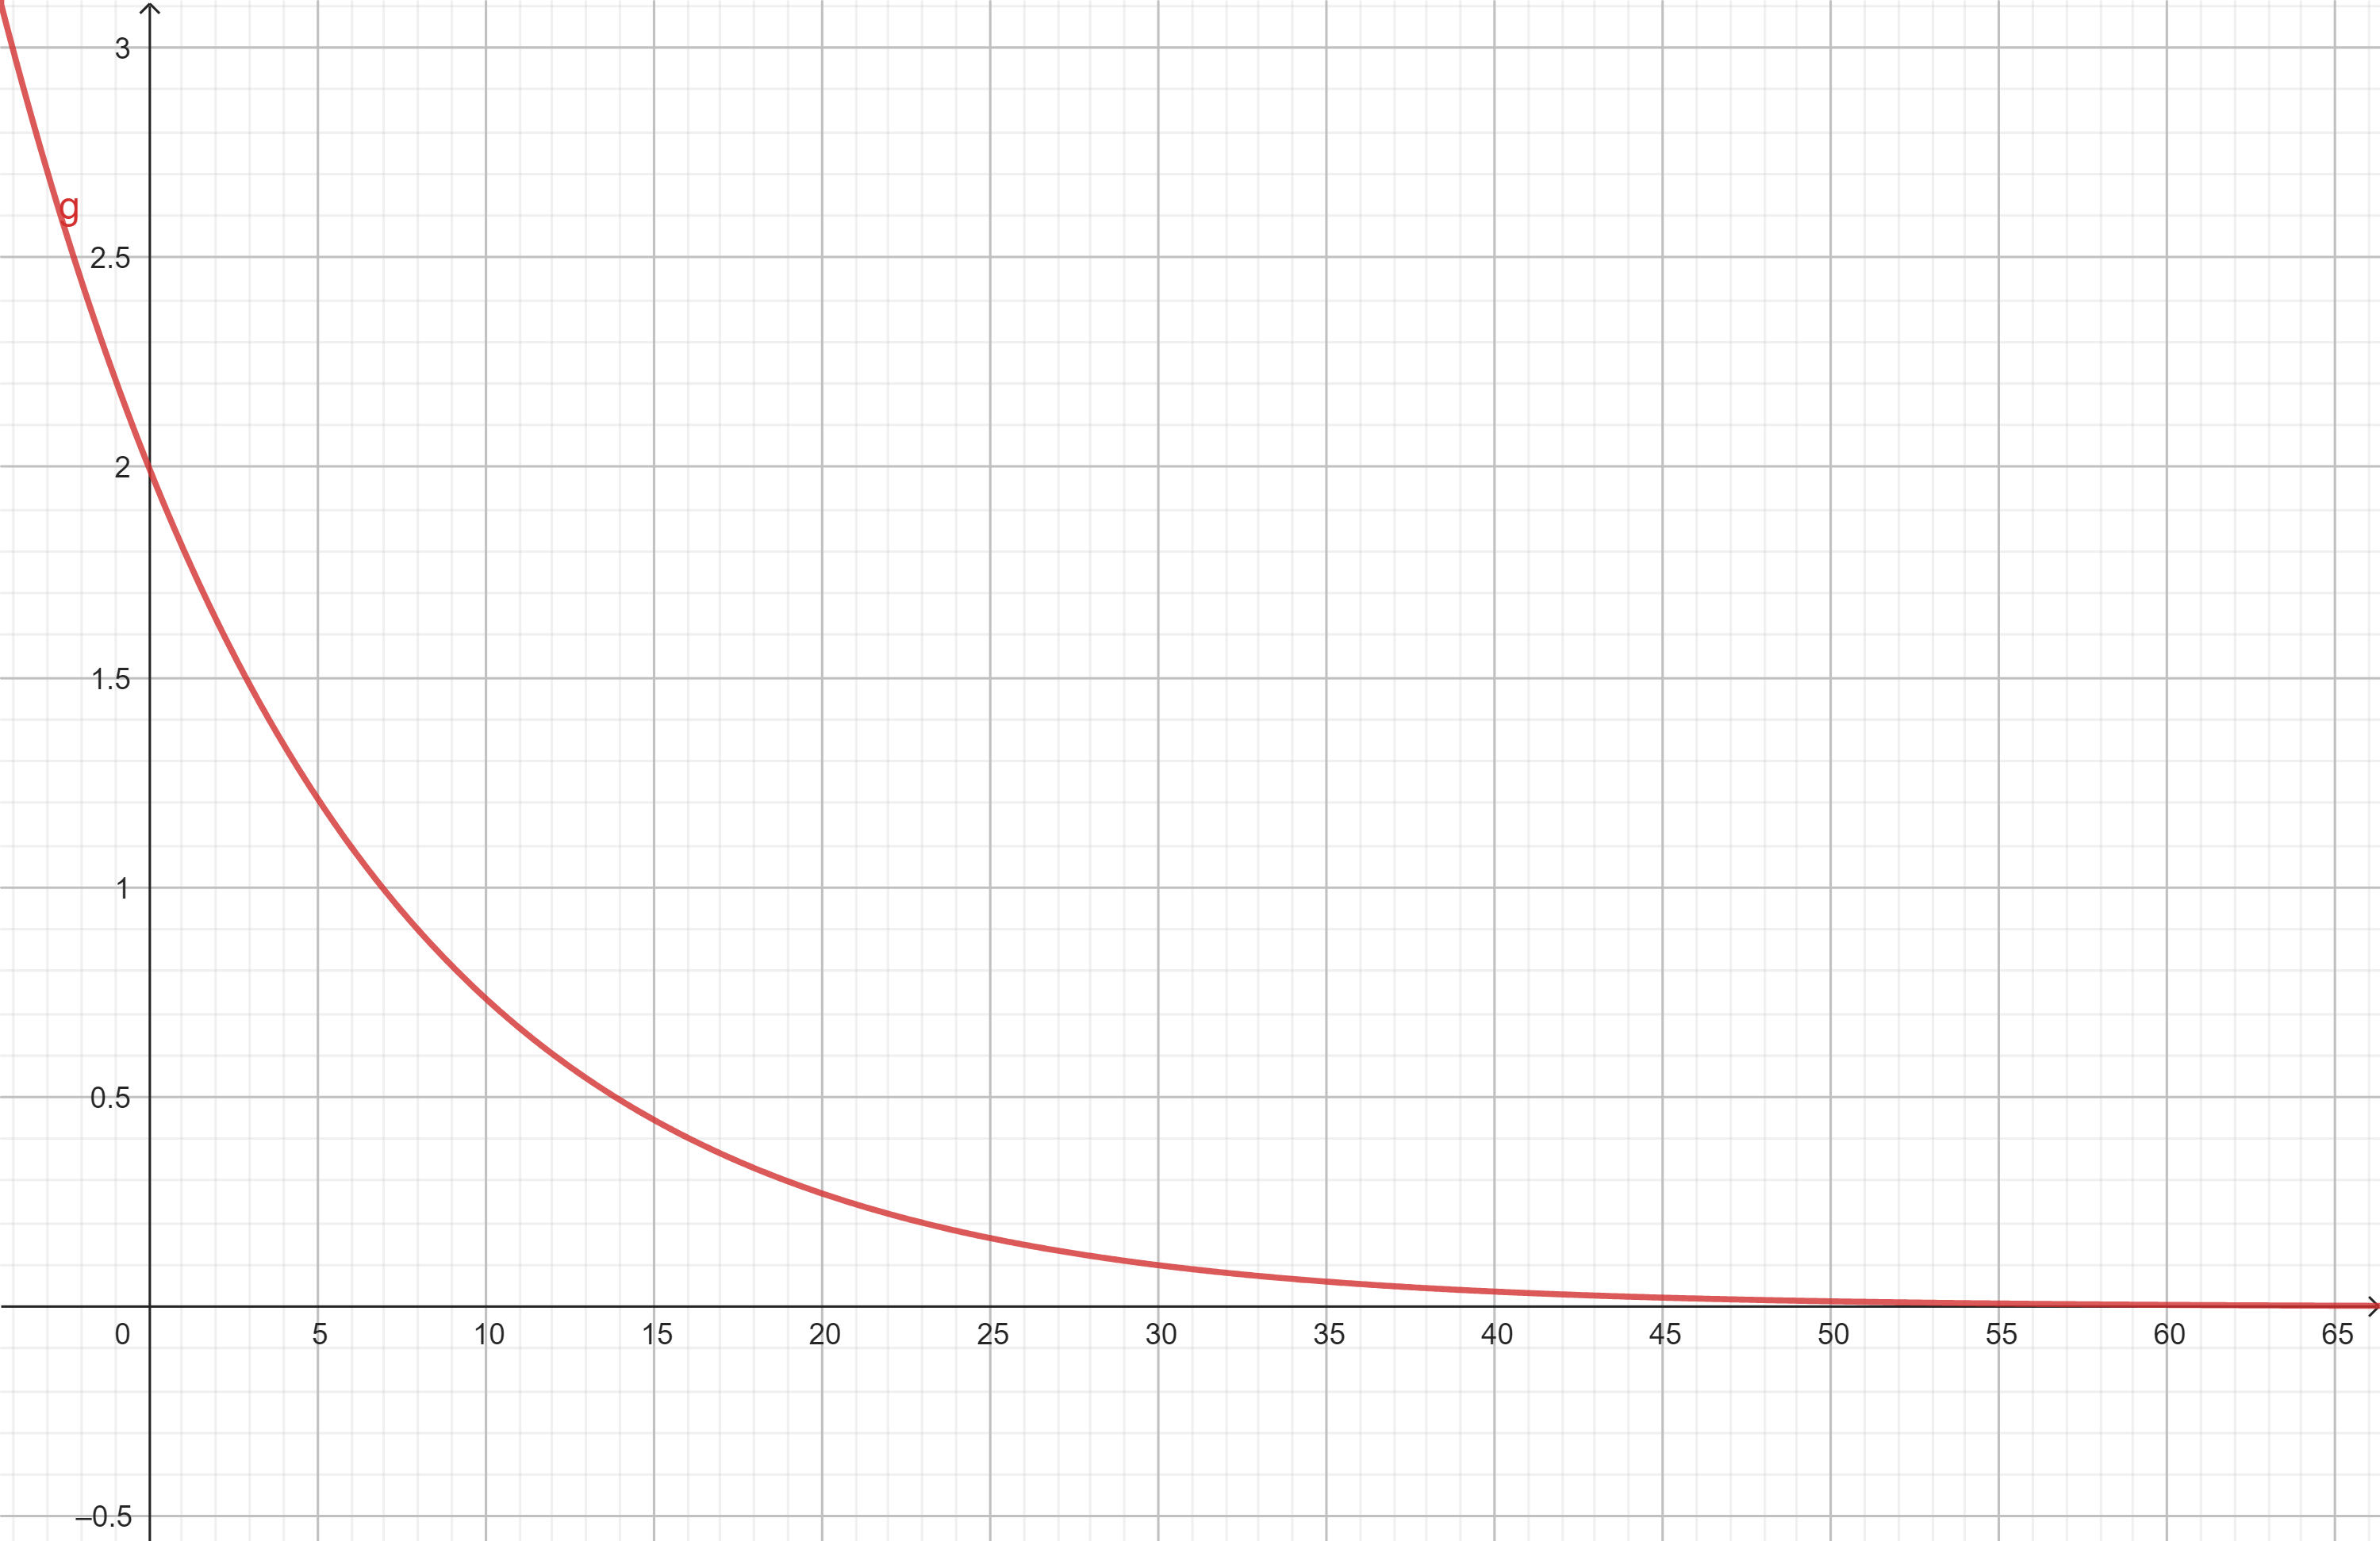
\includegraphics[width=0.8\textwidth]{imagen-ejercicio3.png}
    \caption{Nivel del tanque versus tiempo, simulado en GeoGebra}
\end{figure}

\subsection{Ejercicio 4: Modelo de Población con Migración}

La población de una ciudad cambia según:
\begin{equation}
    \frac{dP}{dt} = -\lambda P
\end{equation}

con $\lambda = 0.05$ año⁻¹ y $P(0) = 100,000$. Determinar cuando la población se reduce a la mitad.

\textbf{Solución:}
La solución es:
\begin{equation}
    P(t) = 100,000 e^{-0.05t}
\end{equation}

Para $P(t) = 50,000$:
\begin{equation}
    50,000 = 100,000 e^{-0.05t} \Rightarrow t = \frac{\ln(0.5)}{-0.05} \approx 13.86 \text{ años}
\end{equation}

\begin{figure}[H]
    \centering
    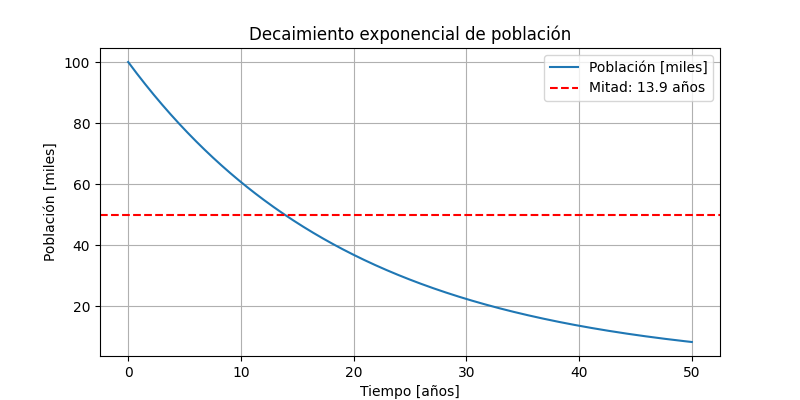
\includegraphics[width=0.8\textwidth]{imagen-ejercicio4.png}
    \caption{Decaimiento exponencial de la población modelado en Python}
\end{figure}

\subsection{Ejercicio 5: Sistema de Segundo Orden Sobreamortiguado}

Resolver:
\begin{equation}
    \frac{d^2 y}{dt^2} + 6 \frac{dy}{dt} + 8y = 0
\end{equation}

con $y(0) = 1$ y $y'(0) = 0$.

\textbf{Solución:}
La ecuación característica es:
\begin{equation}
    r^2 + 6r + 8 = 0
\end{equation}

Las raíces son: $r_1 = -2$, $r_2 = -4$

La solución general es:
\begin{equation}
    y(t) = C_1 e^{-2t} + C_2 e^{-4t}
\end{equation}

Aplicando condiciones iniciales:
\begin{align}
    y(0) &= C_1 + C_2 = 1 \\
    y'(0) &= -2C_1 - 4C_2 = 0
\end{align}

Resolviendo: $C_1 = 2$, $C_2 = -1$

La solución es:
\begin{equation}
    y(t) = 2e^{-2t} - e^{-4t}
\end{equation}

\begin{figure}[H]
    \centering
    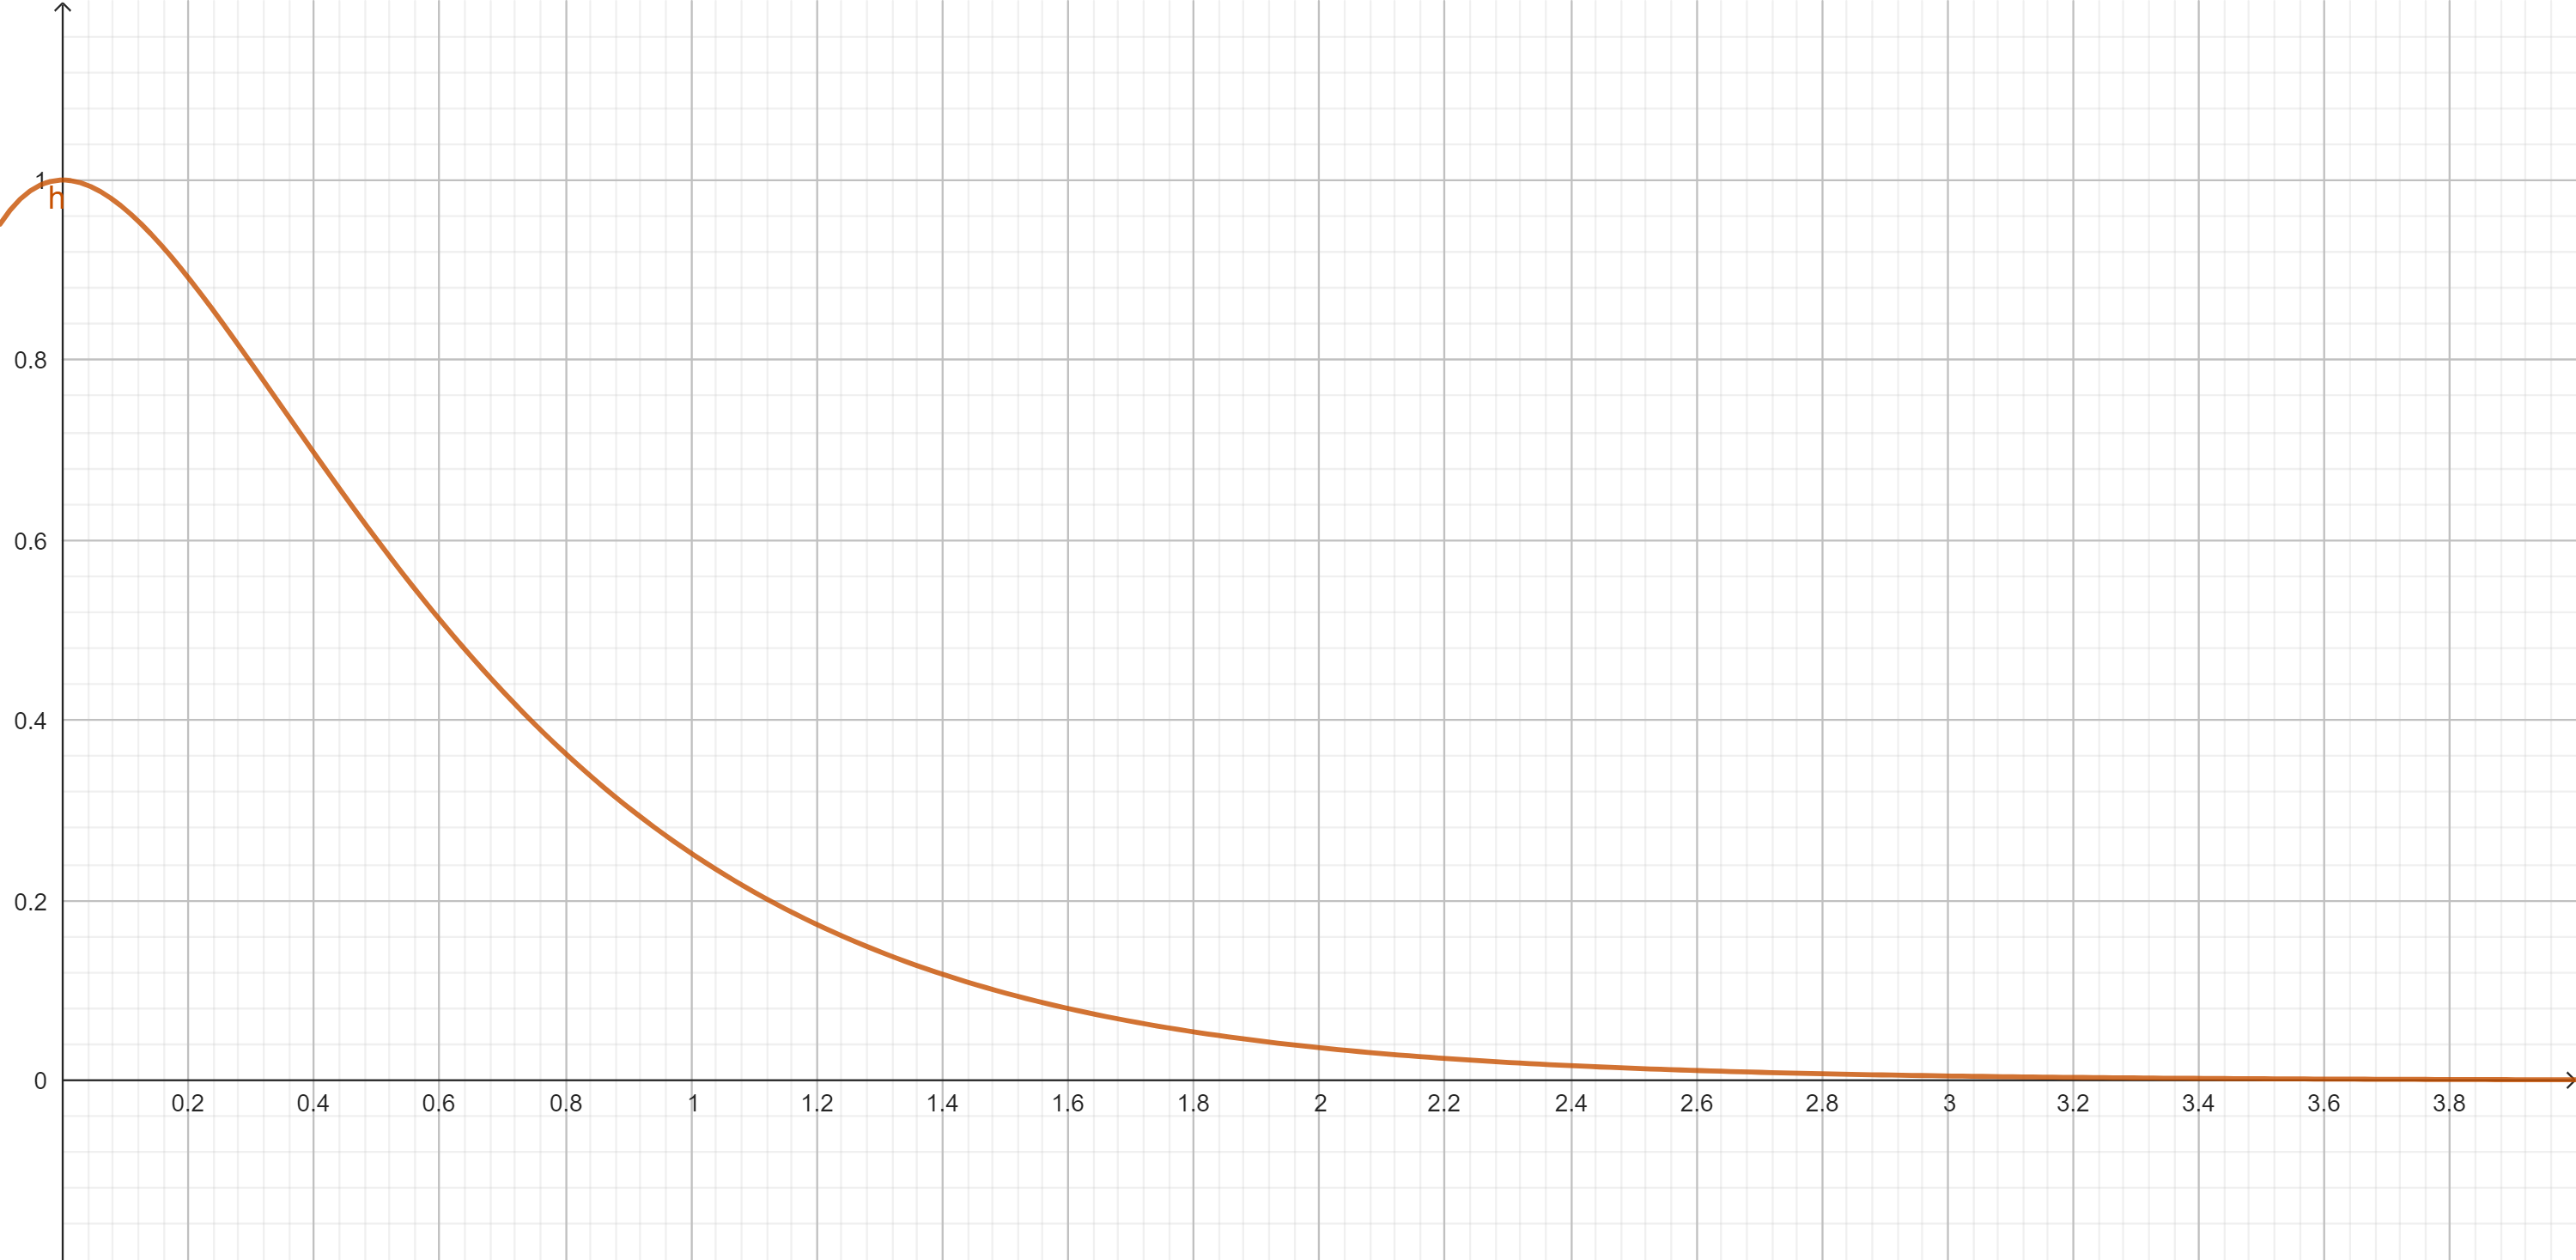
\includegraphics[width=0.8\textwidth]{imagen-ejercicio5.png}
    \caption{Respuesta sobreamortiguada del sistema de segundo orden, simulado en GeoGebra}
\end{figure}

\section{Conclusión}

Las ecuaciones diferenciales homogéneas con coeficientes lineales constituyen una herramienta matemática fundamental para el análisis y diseño de sistemas en Ingeniería de Sistemas. A través de este documento, hemos explorado cómo estas ecuaciones permiten modelar comportamientos dinámicos en diversos contextos, desde sistemas mecánicos y circuitos eléctricos hasta procesos de control y redes de comunicación.

La capacidad de obtener soluciones analíticas para estos sistemas proporciona una ventaja significativa en términos de comprensión y predicción del comportamiento a largo plazo. Los métodos presentados, basados en la resolución de ecuaciones características, ofrecen un enfoque sistemático para analizar la estabilidad, la respuesta transitoria y el comportamiento en estado estacionario de sistemas dinámicos.

Las aplicaciones prácticas demuestran la relevancia de estos conceptos en la resolución de problemas reales de ingeniería. Desde el diseño de sistemas de control automático hasta el análisis de redes de computadoras, las ecuaciones diferenciales homogéneas proporcionan un lenguaje matemático unificado para describir fenómenos temporales complejos.

Para futuras extensiones de este trabajo, sería beneficioso explorar sistemas no homogéneos, ecuaciones con coeficientes variables, y la aplicación de transformadas de Laplace para la resolución de problemas más complejos. Además, la integración de herramientas computacionales modernas permite extender estos análisis a sistemas de mayor dimensión y complejidad, abriendo nuevas posibilidades en el diseño y optimización de sistemas de ingeniería.

\newpage

\section{Referencias}

\begin{thebibliography}{}

\bibitem{boyce}
Boyce, W. E., \& DiPrima, R. C. (2021). \textit{Elementary differential equations and boundary value problems} (12th ed.). John Wiley \& Sons.

\bibitem{zill}
Zill, D. G. (2020). \textit{Ecuaciones diferenciales con aplicaciones de modelado} (11ª ed.). Cengage Learning.

\bibitem{nagle}
Nagle, R. K., Saff, E. B., \& Snider, A. D. (2018). \textit{Fundamentals of differential equations} (9th ed.). Pearson.

\bibitem{ogata}
Ogata, K. (2010). \textit{Modern control engineering} (5th ed.). Prentice Hall.

\bibitem{dorf}
Dorf, R. C., \& Bishop, R. H. (2017). \textit{Modern control systems} (13th ed.). Pearson.

\end{thebibliography}

% recursos.tex
\section{Recursos Adicionales}

\subsection{Enlaces de Interés}

\begin{itemize}
    \item \textbf{Simulaciones de Sistemas Dinámicos:} 
    \url{https://phet.colorado.edu/es/}
    
    \item \textbf{Calculadora de Ecuaciones Diferenciales:} 
    \url{https://www.wolframalpha.com/}
    
    \item \textbf{Tutoriales de GeoGebra:} 
    \url{https://www.geogebra.org/}
    
    \item \textbf{Documentación de Python para Cálculo Científico:} 
    \url{https://docs.scipy.org/doc/scipy/}
\end{itemize}

\subsection{Software Utilizado}

\begin{itemize}
    \item \textbf{GeoGebra:} Software de matemática dinámica para visualización
    \item \textbf{Python con SciPy:} Para solución numérica y gráficos
    \item \textbf{MATLAB/Octave:} Alternativa para simulación de sistemas
\end{itemize}

\subsection{Repositorios de Código}

\begin{itemize}
    \item \textbf{Ejemplos de este documento:} 
    \url{https://github.com/Stirven0/EDOs-Homogeneas}
    \item \textbf{Juego didactico:} 
    \url{https://wayground.com/admin/quiz/68d99f45fc749bfe6872e611}
    
    \item \textbf{Scripts de Python:} Código para generar las gráficas mostradas
    \item \textbf{Archivos de GeoGebra:} Simulaciones interactivas
\end{itemize}

\end{document}